\documentclass[a4paper,10pt]{scrartcl}
\usepackage[utf8]{inputenc}
\usepackage[spanish]{babel} 
\usepackage[hidelinks]{hyperref}
\usepackage{color}
\usepackage{graphicx}
\usepackage{float}
\graphicspath{ {images/} }


\title{Solución al ejercicio Redmine}
\subtitle{Grupo 1.2.2 - Redmine}
\author{
		Manuel Francisco López Ruiz\\
		Julio Márquez Castro\\
		Álvaro Martín Gordillo\\
		  }

\begin{document}

\clearpage\maketitle
\thispagestyle{empty}
\newpage

\newpage

\tableofcontents

\newpage

\section{Crear proyecto}

Crear un nuevo proyecto, llamado "Ejercicio práctico Redmine". Para ello en la pestaña de proyectos, pulsamos en "nuevo proyecto" y rellenamos los campos. Solo tenemos que rellenar "Nombre" y opcionalmente una pequeña "Descripción".\\


	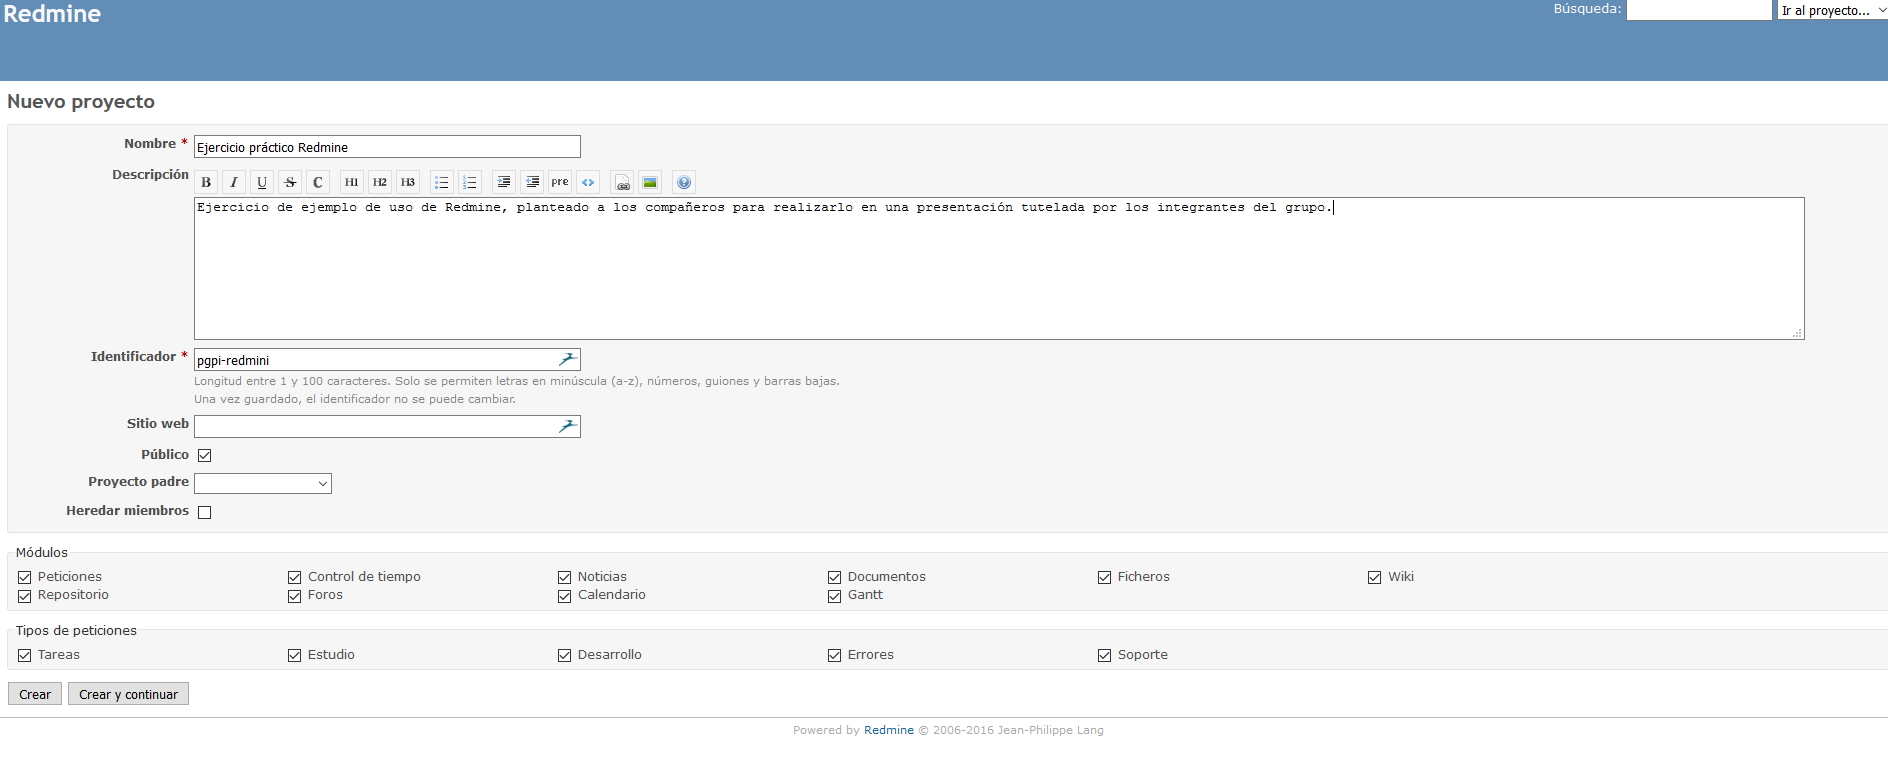
\includegraphics[width=15cm]{crearProyecto}


\section{Incluir miembros}

Para incluir miembros en el proyecto ya creado, vamos a la pestaña de configuración/miembros. Una vez dentro, seleccionamos "Nuevo miembro" y añadimos las cuatro personas integrantes del equipo de trabajo. Tenemos que seleccionar la persona o personas dentro de un mismo perfil(Jefe de Proyecto, Desarrollador...) y añadirlas.\\


	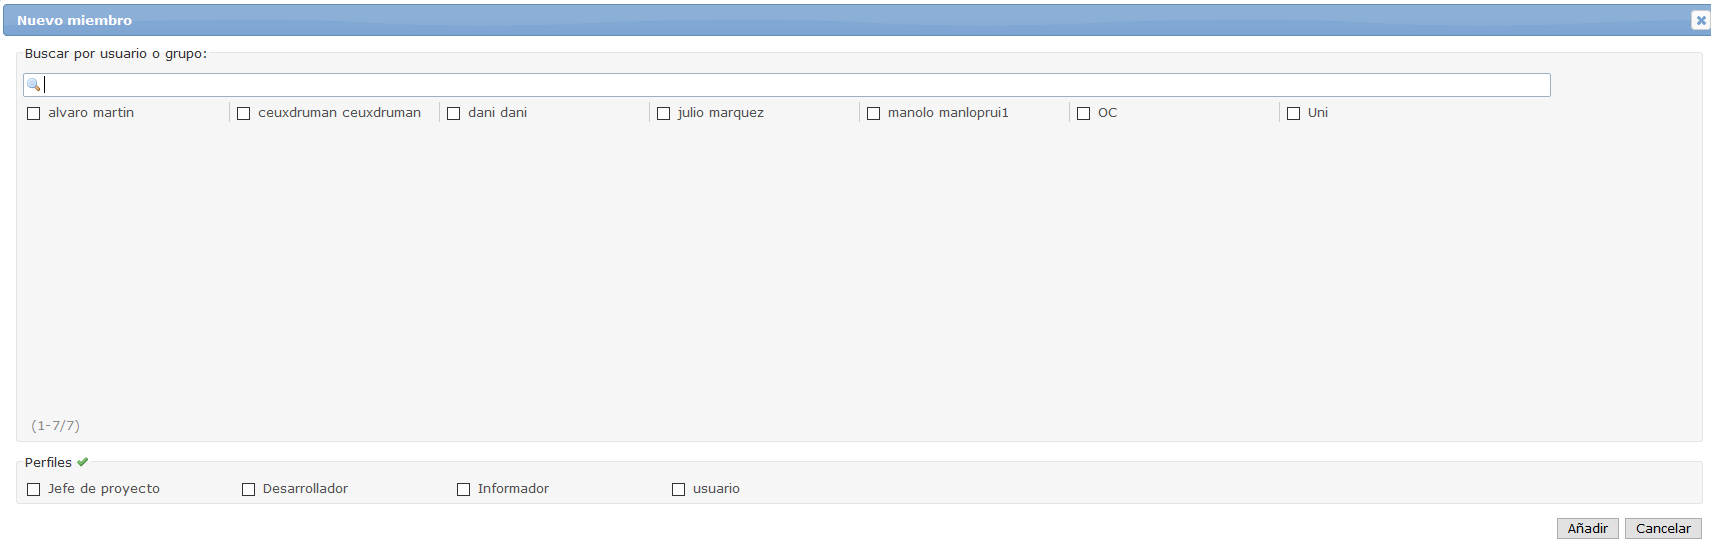
\includegraphics[width=15cm]{AddMiembro}\\

	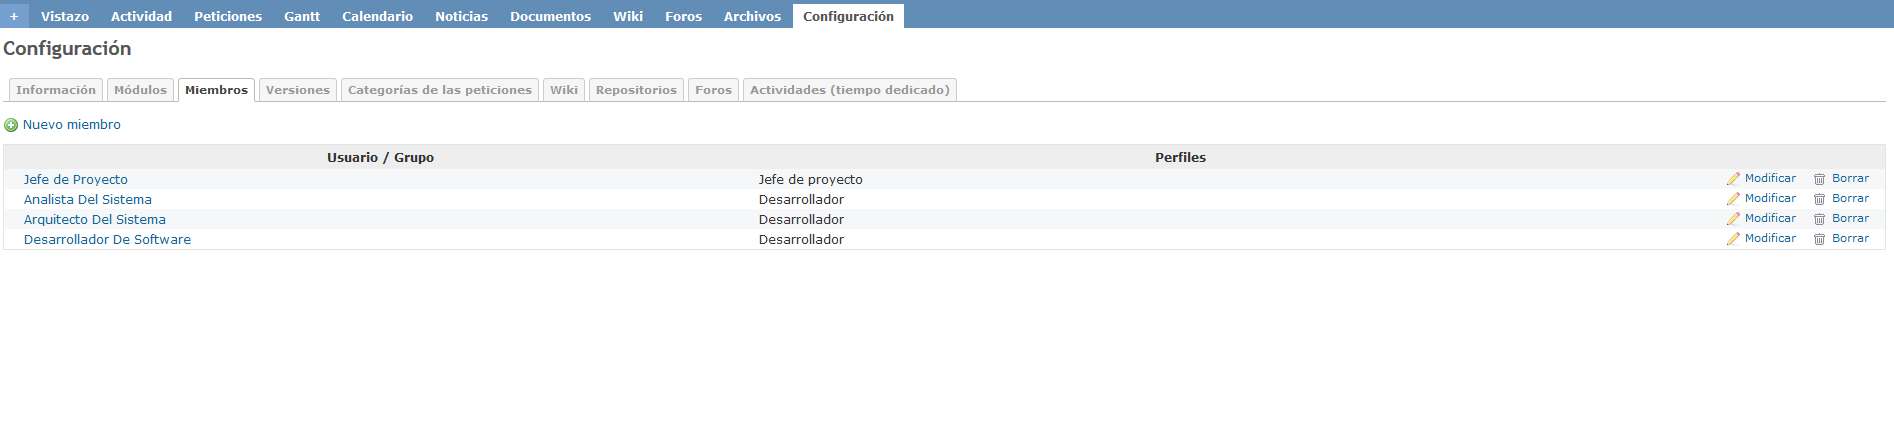
\includegraphics[width=15cm]{Miembros}



\section{Peticiones}

Con los miembros incluidos, pasamos a crear las peticiones/tareas del proyecto. Toda la información necesaria esta en el enunciado del ejercicio, con algunas cosas a tener en cuenta. Como la fecha de inicio de las peticiones, para las tareas 1, 1.1, 1.2, 1.3 es la misma fecha de inicio del proyecto(05/09/2016), pero para las tareas restantes la fecha de inicio debe ser el mismo o un día después de finalizar la tarea antecesora.\\

Para crear una petición, en la pestaña de peticiones, pulsamos en "Nueva Petición" y rellenamos los campos con los datos proporcionados en el enunciado. Para crear subtareas, debemos quedarnos con el código identificador de la tarea padre, o entrar en los detalles de la tarea padre, pulsando sobre ella en la lista de tareas, y pulsar en el botón de "añadir" en el apartado de subtareas.\\

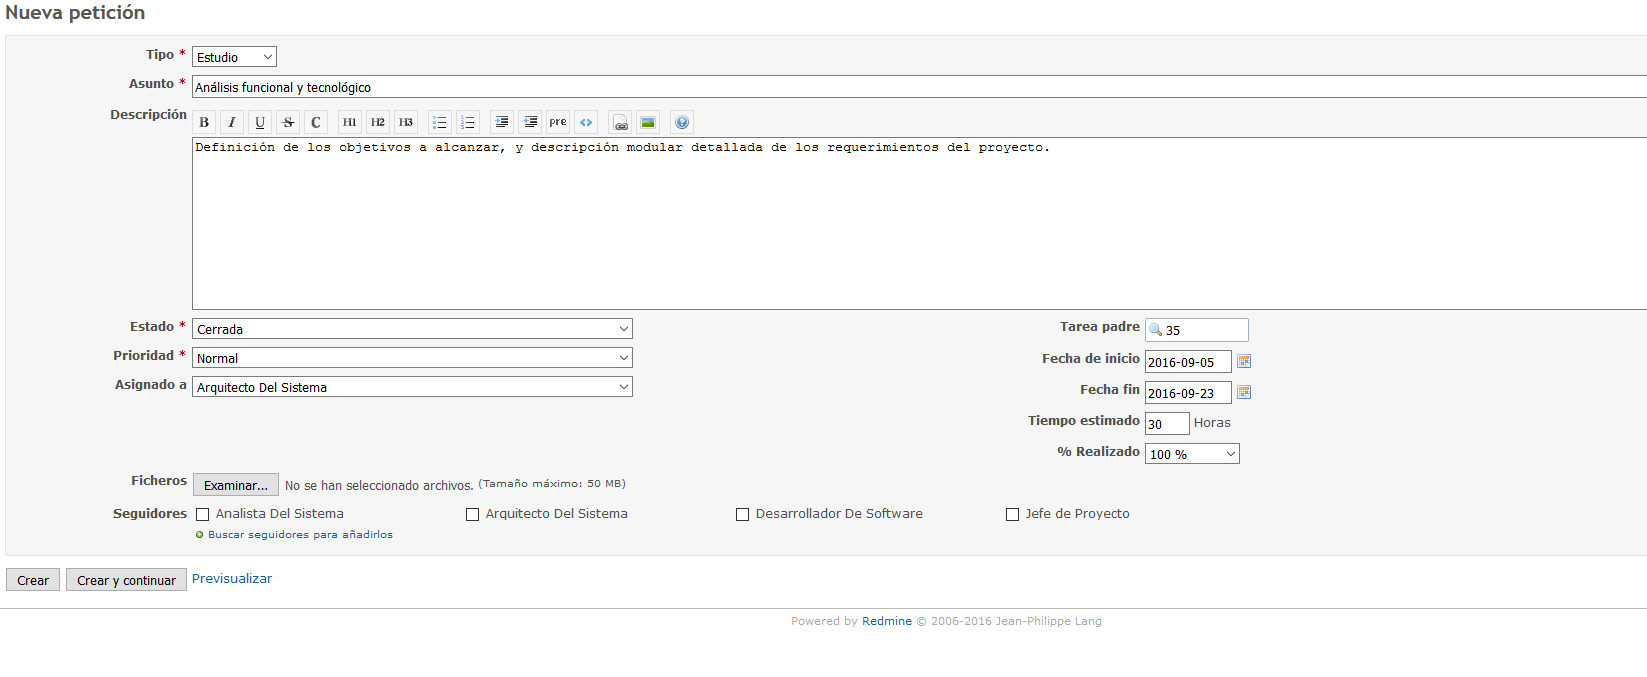
\includegraphics[width=\linewidth]{NuevaPeticion}\\

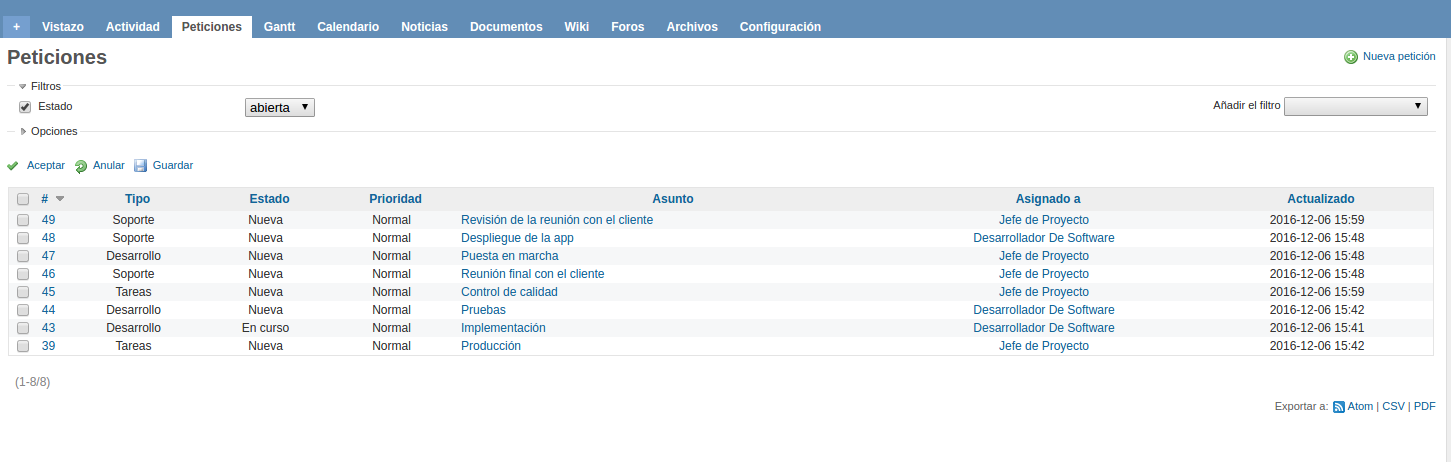
\includegraphics[width=\linewidth]{peticiones}

\section{Foros}

Para crear el foro pedido en el enunciado, debemos ir a la pestaña Configuración/Foros y pulsar el enlace a "Nuevo Foro". Rellenamos los campos con los datos del enunciado y pulsamos en "Crear".\\

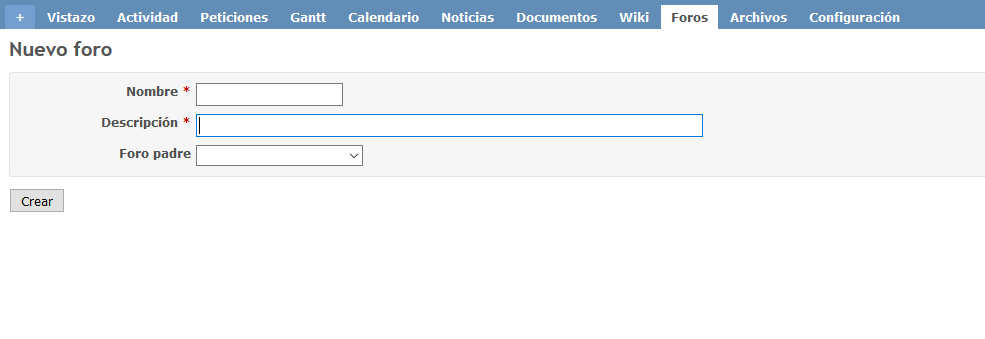
\includegraphics[width=\linewidth]{NuevoForo}\\

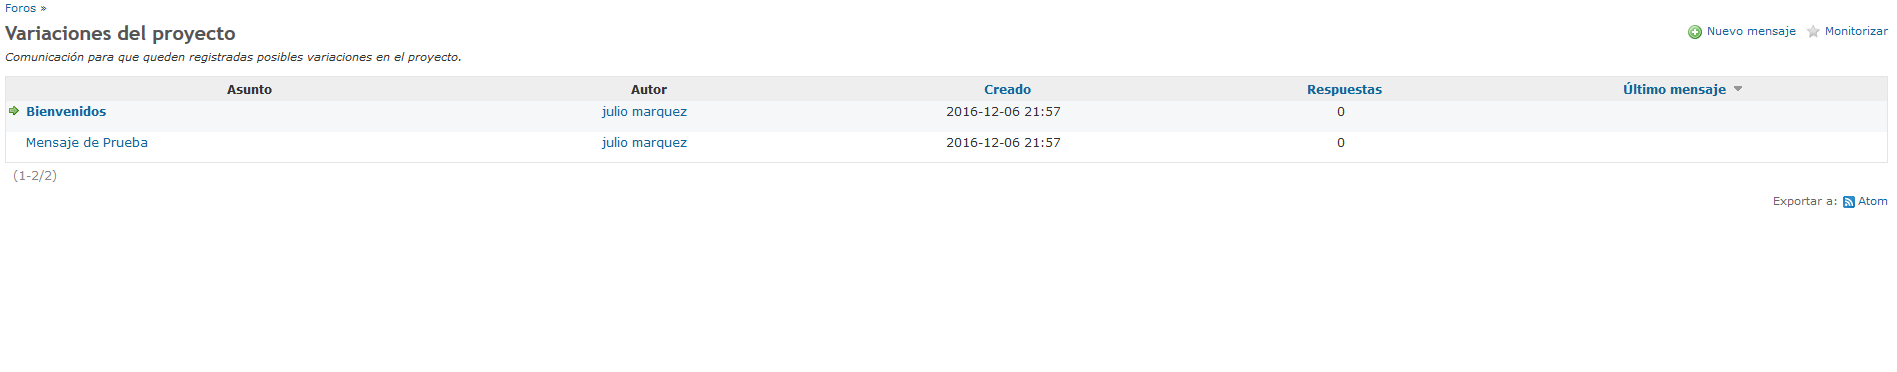
\includegraphics[width=\linewidth]{Foros}

\subsection{Mensaje de bienvenida}

Para crear el mensaje de bienvenida, debemos ir a la pestaña Foros(inicialmente no debe verse esta pestaña hasta que no creemos un foro). Si solo tenemos un foro, accederá automáticamente a este, en caso contrario debemos seleccionar el foro de "Variaciones del proyecto" y pulsar en "Nuevo mensaje". Rellenamos los campos de Asunto y el mensaje y marcamos las casillas de pegajoso y bloqueado para dejar el mensaje fijado.\\
\\

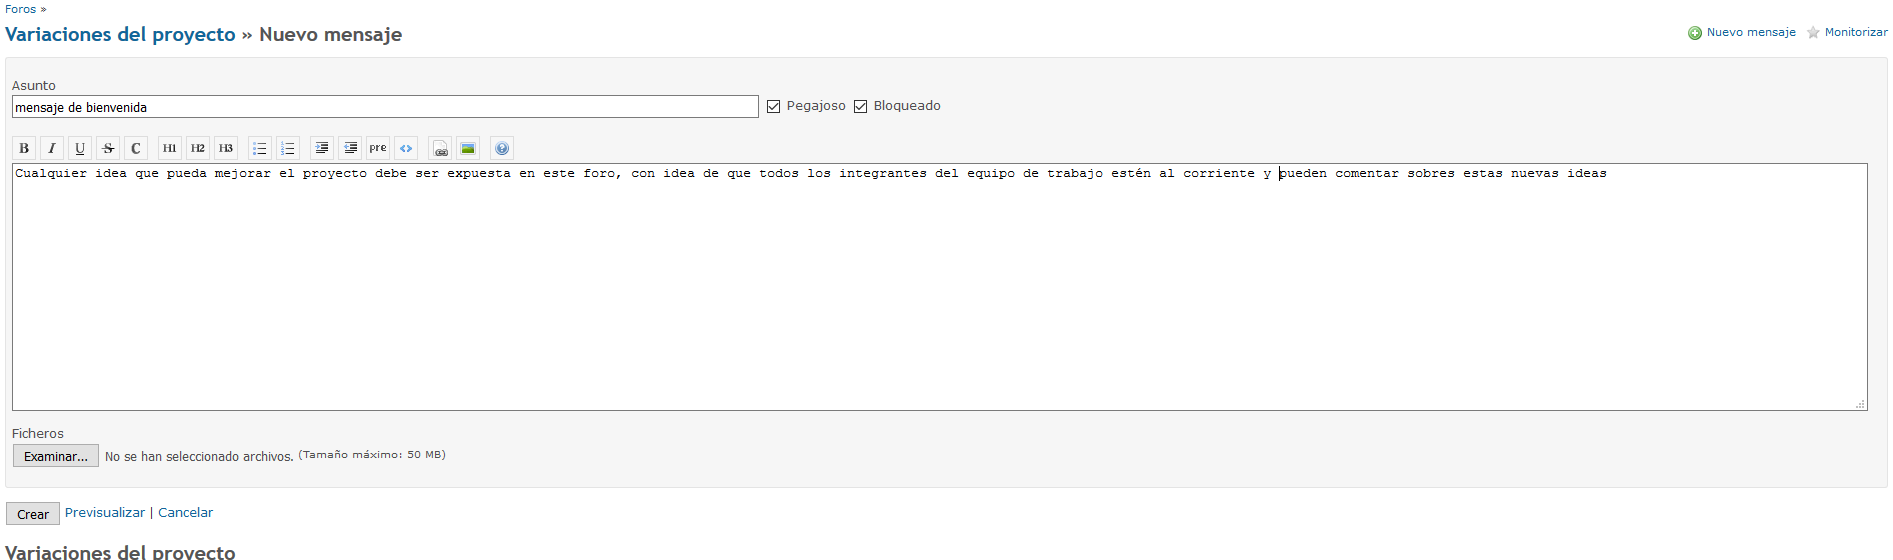
\includegraphics[width=\linewidth]{NuevoMensaje}

\newpage
\section{Gantt}

Una vez creada todas las tareas del proyecto podemos acceder a la pestaña de Gantt y podemos ver el diagrama de Gantt del proyecto.\\

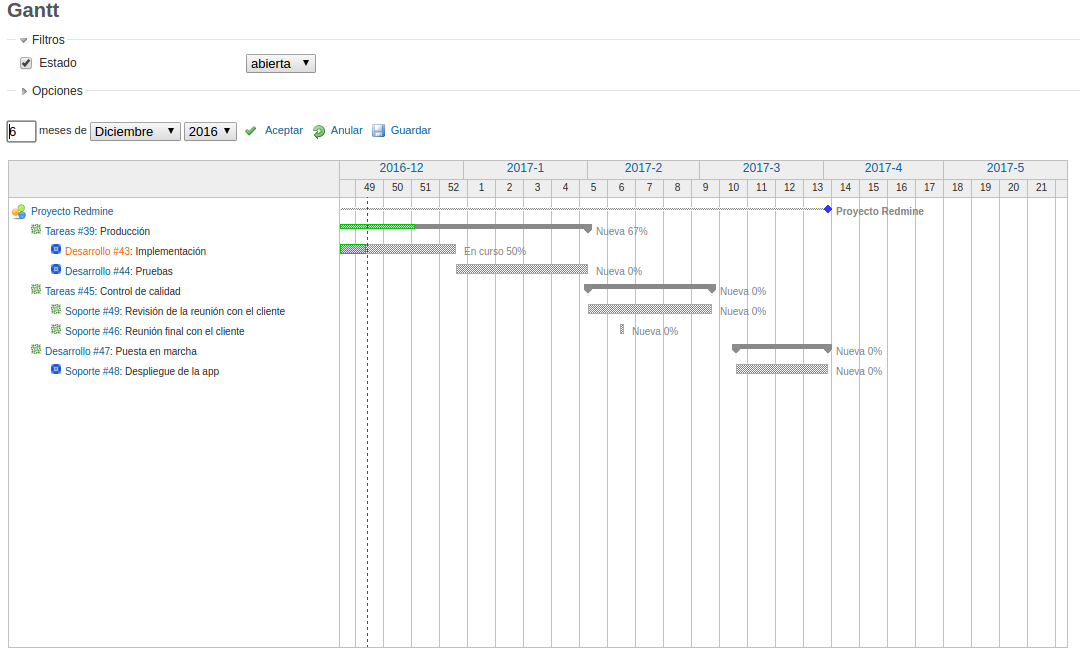
\includegraphics[width=\linewidth]{gantt}

\bibliography{sample}

\end{document}
